\documentclass[11pt, a4paper]{article}

\usepackage{amsmath}
\usepackage{amsfonts} %Matheschriften
\usepackage{amssymb} %Mathesymbole
%\usepackage{mathptmx} % Einstellung für Schriften und Sonderzeichen in mathematischen Umgebungen
                        % ändert SChriftfont
\usepackage{wasysym} % Stellt diverse Sonderzeichen bereit
\usepackage{siunitx}
\usepackage{float}
\usepackage{microtype}
\usepackage{graphicx}
\usepackage{hyperref}
\usepackage{xcolor}
\usepackage[section]{placeins}


\usepackage[ngerman]{babel}
\addto\captionsngerman{%
 \renewcommand{\abstractname}{Abstract}}

\title{Versuch 3: Schiefe Ebene}
\author{Jascha Fricker, Benedict Brouwer}

\begin{document}
    \maketitle

    

    \begin{abstract}
        Schon Gallileo hat mit schiefen Ebenen experiemtiert und auch heute ist die schiefe Ebene ein viel benutztes
        Modell. Auch in diese Versuch betrachten wir eine Schiefe Ebene, messen die Kraftkomponenten und
        die Reibung. 
    \end{abstract}

    \tableofcontents

    \newpage

    \section{Kräftezerlegung}
    \subsection{Theorie \& Experimenteller Aufbau}
    Bei einer schiefen Ebene zerlegt sich die wirkende Gravitationskraft in zwei Teilkräfte.
    \begin{align}
        \text{ Normalkraft } \ \ F_\perp = F_g cos \alpha \\
        \text{ Tangentialkraft } \ \ F_\parallel = F_g sin \alpha 
    \end{align}
    Im Experiemt werden diese Kräfte mit zwei Kraftmessern für unterschiedliche Winke $\alpha$ bestimmt.

    \subsection{Ergebnisse \& Diskussion}
    \begin{figure}
        \centering
        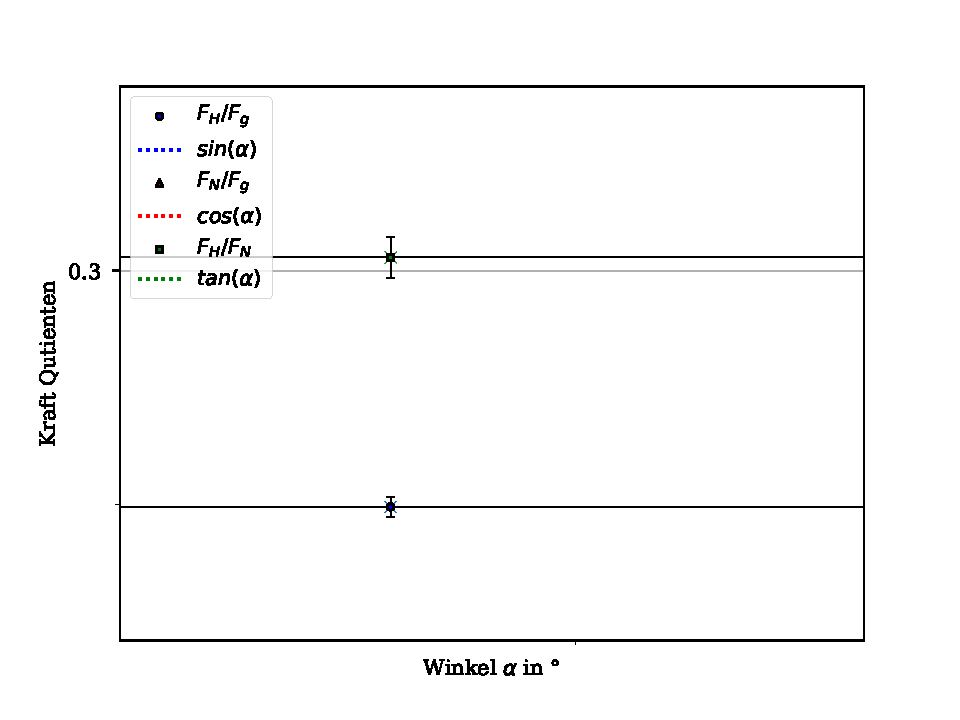
\includegraphics[width=100mm]{./5Kraftzer.pdf}

        \caption{Kraftquotienten der Kräftezerlegung}
        \label{fig:Kraftzer}
    \end{figure}
    Im Graph \ref{fig:Kraftzer} sind die die berechneten Kraftquotienten bezüglich der verschiedenen Winkel aufgetragen.
    Es kann erkannt werden, dass die Messwerte sehr stark von den Theoriekurven abweichen, dies liegt wahrscheinlich
    am ungenauen Versuchsaufbau.
    
    In diesem Versuch wurden die Unsicherheiten des Kraftmessers(Schrittweite), die Unsicherheit der Waage($1\si{\gram}$)
    sowie die Unsicherheiten der Winkelmessung(Schrittweite $1 \si{\milli\metre}$) berücksichtigt.
    Durch den Versuchsaufbau konnte nicht verifiziert werden, dass die Normalkraft genau senkrecht anliegt.
    Anhand der Daten lässt sich ein Unsicherheitintervall von etwa $3,5^{\circ}$ ableiten, welches auch zu
    Beobachtungen bei der Versuchsdurchführung passt. Für die Unsicherheiten wurde erst der Mittelwert \cite[(29)]{ABW} mit
    und die Standardabweichung mithilfe der Student-t-Verteilung \cite[(15)]{ABW} der beiden Kräfte berechnet, um dann mithilfe der Gausschen
    Gausschen Fehlerfortpflanzung \cite[(19)]{ABW} die Unsicherheit der Quotienen zu berechnen.

    \section{Haftreibung}
    \subsection{Theorie \& Experiemteller Aufbau}
    Die Haftreibung ist die Reibungskraft, die existiert, wenn ein Körper sich nicht bewegt.
    Die Haftreibungskraft
    \begin{align}
        F_H = \mu_H \cdot F_n
    \end{align}
    ist proportional zur Normalkraft und zur Haftreibungskonstante $\mu_H$. Um diese zu messen,
    wird mit einem Kraftmesser tangential Kraft an die Masse angelegt. Diese wird langsam erhöht.
    Sobald die Masse anfängt zu rutschen, wird die direkt vorher angelegt Kraft als Haftreibungskraft notiert.

    \subsection{Ergebnis \& Diskussion}
    In Graph ? kann anhand der Steigung der Ursprungsgerade der Haftreibungskoeffizient
    \begin{align}
        \mu_H = 0,155(87)
    \end{align} 
    bestimmt werden.
    Die große Abweichung der einzelnen Messungen liegt wahrscheinlich an der Inhomogenität der Haftreibung
    abhängig vom Ort, an dem gemessen wurde. Auch beim 3. Versuch haben wir diesen Effekt
    bei der Gleitreibung bei kleinen Winkeln bemerkt. Der Fehler wurde durch programmatisches Ausrechnen von
    $\mu_H$ für jeden einzelnen Punkt und anschließendem bestimmmen der gewichteten Mittelwerts mit
    Ungenauigkeit \cite[(29)]{ABW} berechnet. 

    \section{Gleitreibung}

    \subsection{Theorie \& Experiemteller Aufbau}

    Die Gleitreibung ist im Gegensatz zur Haftreibung die Reibung, die entsteht, während der Körper gleitet.
    Wenn ein Körper eine schiefe Ebene hinuntergleitet, hat er folgende Bewergungsgleichung:
    \begin{align}
        \text{ohne Reibung:} \ \  s(t) &= \frac{g \cdot sin(\alpha)}{2} \cdot t^2 +v_0 \cdot t + x_0 \\
        \text{mit Reibung:} \ \  s(t) &= g \cdot \frac{sin(\alpha) -\mu_G cos(\alpha)}{2} \cdot t^2 +v_0 \cdot t + x_0
    \end{align}
    Aus der 2. Ableitung $a$ der Theorieparabel kann die Gleitreibungskonstante
    \begin{align}
        &a = g \cdot (sin(\alpha) - \mu_G cos(\alpha)) \\
        &\Rightarrow \ \ \mu_G = tan(\alpha) \cdot \frac{a}{g}
    \end{align} 
    berechnet werden




    \bibliographystyle{plain}
    \bibliography{literature}

\end{document}